\section{Sliding Window Methods}


\section{Graph-based Methods}
As mentioned earlier, graph-based segmentation approaches construct connected components using weighted edges between the vertices (pixels). The \emph{Felzenszwalb} algorithm is a graph-based algorithm that tries to discover the connected components of a graph in a hierarchical fashion.
More formally, let $G = (V, E)$ be a graph where each $v_i \in V$ represents a pixel in the image and every undirected edge $\{v_i, v_j\} \in E$ connects a pair of neighbouring pixels. Each edge is associated with a non-negative weight $w(\{v_i, v_j\})$ that corresponds to a dissimilarity measure between the two pixels.
The algorithm tries to partition the vertex set $V$ into a set of disjoint nonempty components (regions) $S = \{C_1, \ldots C_k\}$ such that the edge weights between two points in the same components are relatively low compared to the edge weights between points in different components.

\begin{figure}[ht]
    \centering
    \includegraphics[width=.9\linewidth]{figures/felzenszwalb_results.pdf}
    \caption{Three images segmented using the Felzenszwalb algorithm with d=50 (left), 300 (middle), 1000 (right).}
    \label{fig:felzenszwalb_results}
\end{figure}

The algorithm starts by placing each pixel in its own component. It then proceeds by visiting each edge and merging the components of the two edge endpoints (should the two endpoints lie in different components) based on an evidence predicate. The evidence predicate states whether two components should remain disconnected or be merged into one larger component. It compares the difference between the two components in question against the internal difference within each component. The internal difference of a component $C$ is defined as:
\begin{equation}
    \varphi(C) = \max_{e \in MST(C,E)}(w(e))
\end{equation}
where $MST(C,E)$ is the minimum spanning tree required to span component $C$. A low internal difference value would indicate that the component is dense (since the component's members have a low maximum dissimilarity with respect to the MST).
The inter-component difference between two components is a measure of how distanced the two components are. It is defined as:
\begin{equation}
    \psi(C_1, C_2) = \min_{v_i \in C_1, v_j \in C_2, \{v_i, v_j\} \in E}w(\{v_i, v_j\})
\end{equation}
A high inter-component difference between two components would indicate the two components are highly dissimilar. The evidence predicate compares the two aforementioned measures as follows:
\begin{equation}
    P(C_1, C_2) = 
    \left\{
	\begin{array}{ll}
		\mbox{True}  & \mbox{if } \psi(C_1, C_2) > \min(C_1 + \tau(C_1), C_2 + \tau(C_2))\\
		\mbox{False} & \mbox{otherwise}
	\end{array}
\right.
\end{equation}
where $\tau(C) = \frac{d}{|C|}$ is a threshold parameter for some constant $d$.
If the predicate evaluates to true, then a boundary is present between the two components and they remain disconnected. This is due to the fact that the inter-component difference (which indicates the closest two points between the two components) is greater than the internal difference of either component. The threshold parameter controls the amount of evidence needed for a drawing a boundary between the two components. Increasing the value of $d$ in $\tau(C)$ corresponds to increasing the minimum requirement for building a boundary between the two components and hence, results in larger segments in the final segmentation result.
\autoref{fig:felzenszwalb_results} shows the results for different values of $d$. The figure shows that increasing the value of $k$ increases the size of the superpixels generated.

%%%%%%%%%%%%%%%%%%%%%%%%%%%%%%%%%%%%%%%%%

As mentioned in the beginning of this chapter, we intend to perform the clustering in the feature space. However, since the vectors of the feature tensor are several hundred channels deep, clustering the feature vectors directly might not always yield optimal results. This is due to the fact that data is sparse in very high dimensional space. The data is said to suffer from the \emph{curse of dimensionality}. In order to address this problem, we reduce the dimensionality of the vectors in the tensor of features to aid the subsequent clustering step. Afterwards, we outline a method for automatically choosing the number of clusters.

The final step is choosing the number of principal components required to represent our data. This can be done by plotting the principal components against the percentage of the variance that they capture. Afterwards, the number of principal components is chosen according to the elbow of the plot.

As part of understanding what the principal components mean, we apply PCA to the vectors of the output tensor of features. The output was taken from the deepest convolutional layer of the network (layer 29). \autoref{fig:first_pc} shows single channel images where each pixel is colored by the value of the first principal component of its corresponding feature vector. The results show that the first principal component can sometimes separate the foreground from the background in some images. Moreover, they show that the model has gained a deeper understanding of the objects in the image beyond the notion of color.

\begin{figure}[!ht]
    \centering
    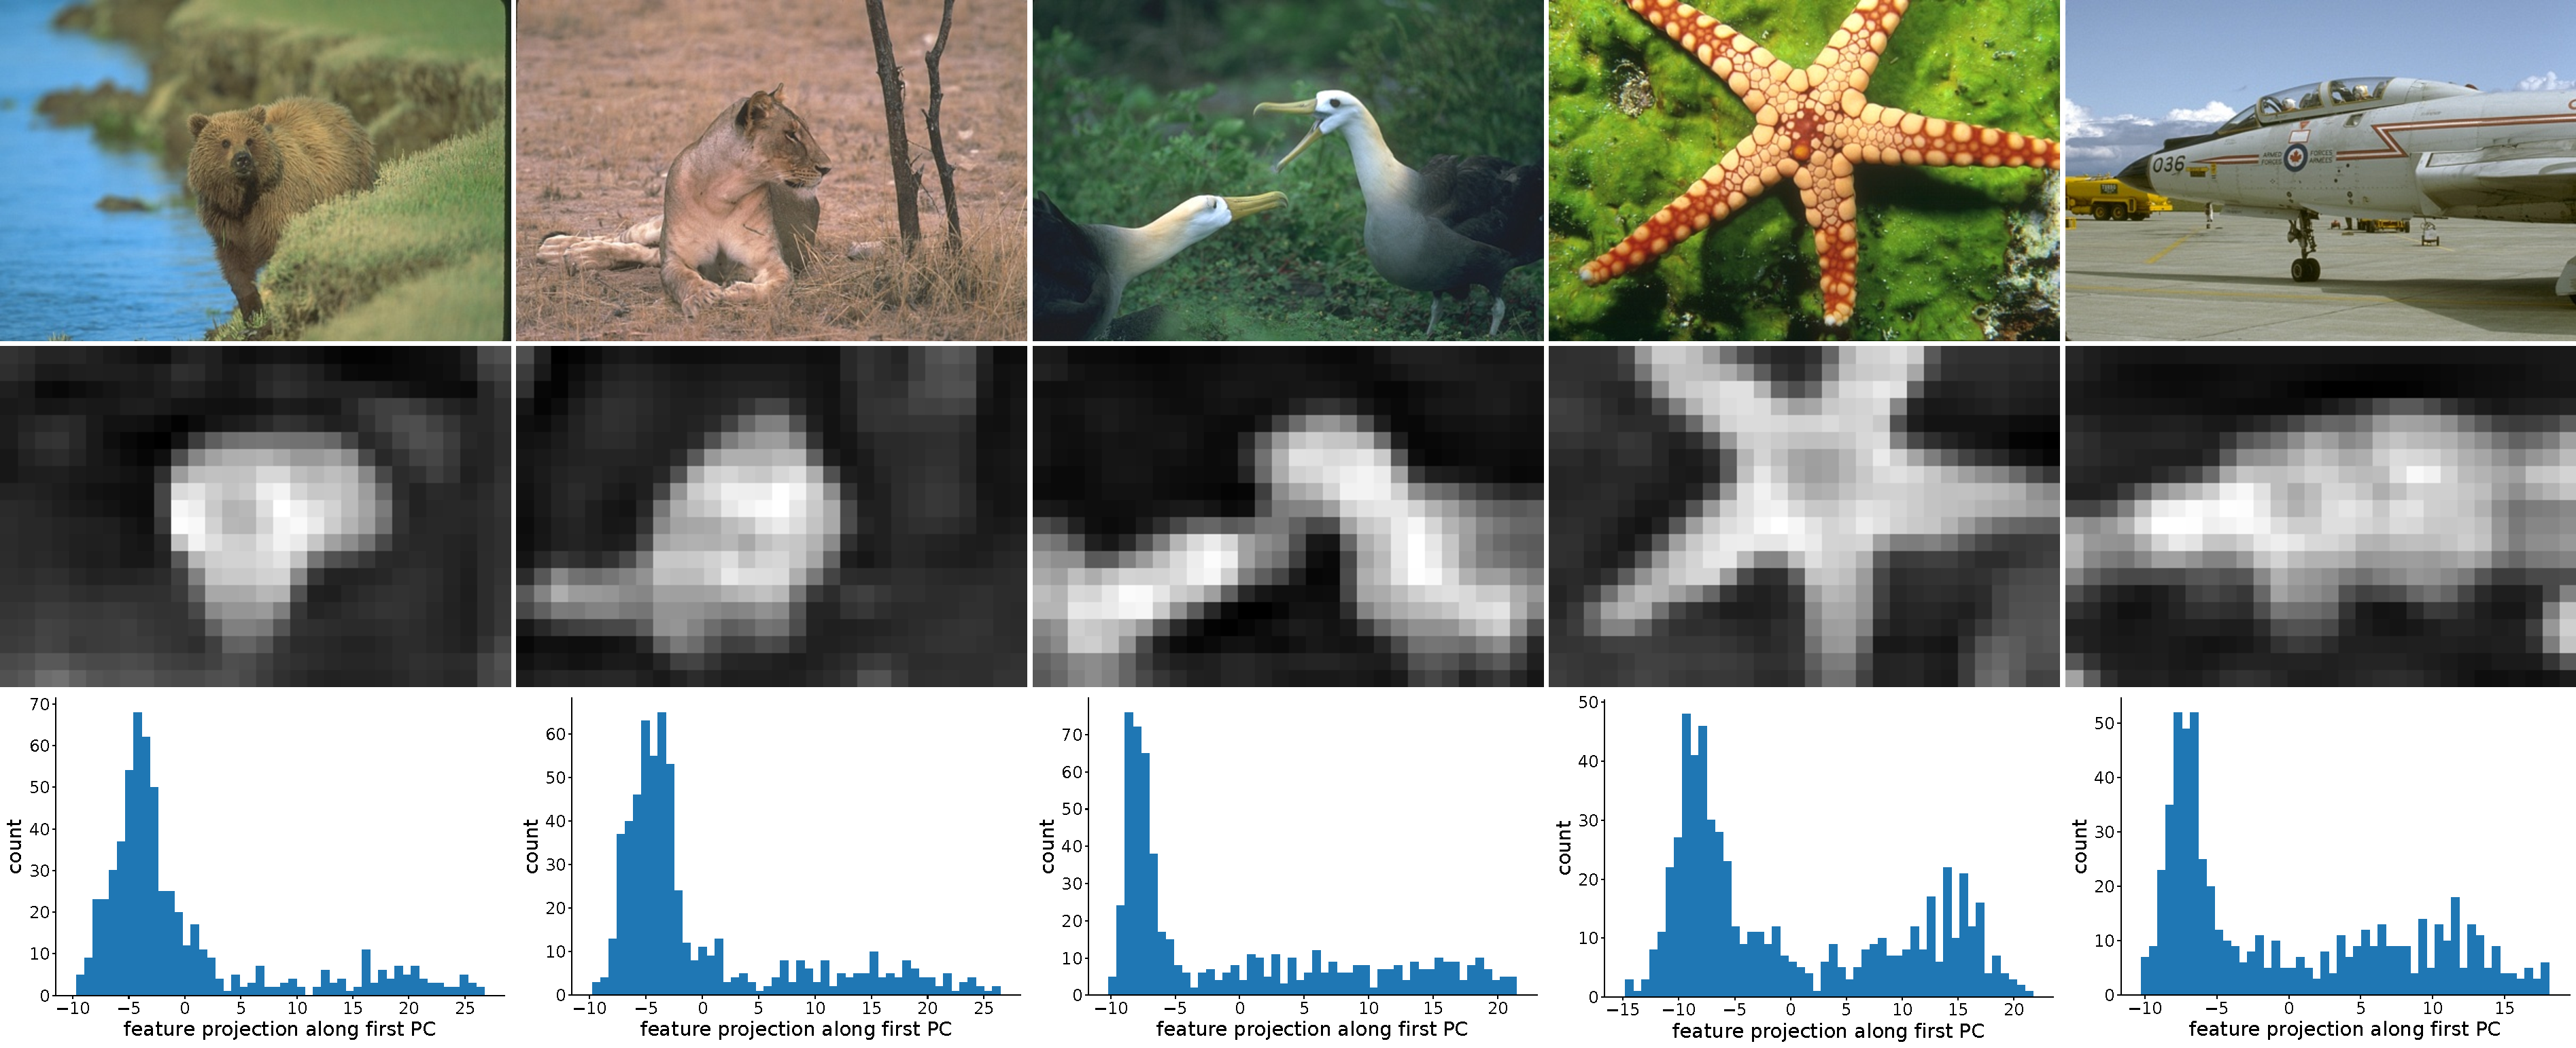
\includegraphics[width=\linewidth]{figures/first_pc.pdf}
    \caption{Images from BSD500 \parencite{bsd500} (1\textsuperscript{st} and 3\textsuperscript{rd} column) are passed down VGG16. Each output tensor is extracted from the deepest convolutional layer and processed using PCA individually. The grayscale image representation of the first principal component (2\textsuperscript{nd} and 4\textsuperscript{th} column) can sometimes separate the foreground objects from the background. Brighter pixels have a greater value than darker pixels.}
    \label{fig:first_pc}
\end{figure}

After reducing the dimensionality of the feature tensor, similar feature vectors are clustered together to obtain a final segmentation. Since we plan to use the k-means algorithm (see \autoref{section:k-means}), an appropriate cluster number needs to be determined.

\begin{figure}[ht]
    \centering
    \includegraphics[width=\linewidth]{figures/silhouette_scores.pdf}
    \caption{Results obtained by clustering images in their feature space. The original images (left) are clustered in feature space using k-means. The number of clusters in the final segmentation (middle) is chosen as the value which maximizes the silhouette index in a predefined interval (right). Each region is colored by the average color of the pixels in that region.}
    \label{fig:silhouette_scores}
\end{figure}

%%%%%%%%%%%%%%%%%%%%%%%%%%%%%%%%%%%%%%%%%%%%%%%%%%%%%%%%%%%%%%%%%%%%
%%%%%%%%%%%%%%%%%%%%%%%%%%%%%%%%%%%%%%%%%%%%%%%%%%%%%%%%%%%%%%%%%%%%
%%%%%%%%%%%%%%%%%%%%%%%SMV%%%%%%%%%%%%%%%%%%%%%%%%%%%%%%%%%%%%%%%%%%
%%%%%%%%%%%%%%%%%%%%%%%%%%%%%%%%%%%%%%%%%%%%%%%%%%%%%%%%%%%%%%%%%%%%
%%%%%%%%%%%%%%%%%%%%%%%%%%%%%%%%%%%%%%%%%%%%%%%%%%%%%%%%%%%%%%%%%%%%
%%%%%%%%%%%%%%%%%%%%%%%%%%%%%%%%%%%%%%%%%%%%%%%%%%%%%%%%%%%%%%%%%%%%

\section{Contour Refinement Using Superpixels}

Chapter \ref{chapter:clustering_in_feature_space} explored segmenting feature images. One disadvantage of using the feature images is that they have a lower spatial resolution than the original image. This is due to the downsampling caused by the max pooling layers in the CNN architecture. As a result, accurate boundary information between two adjacent regions is lost. The lower resolution segmentation image does not have enough pixels to represent the different contours accurately. Some methods have been proposed in the literature for reusing the color superpixel image to further refine the final segmentation \parencite{ma2018fully}. In this subsection, we investigate restoring some of the original contours of the segmentation image by using the superpixel color image. \autoref{fig:smv} outlines the process described in this subsection.

\begin{figure}[ht]
    \centering
    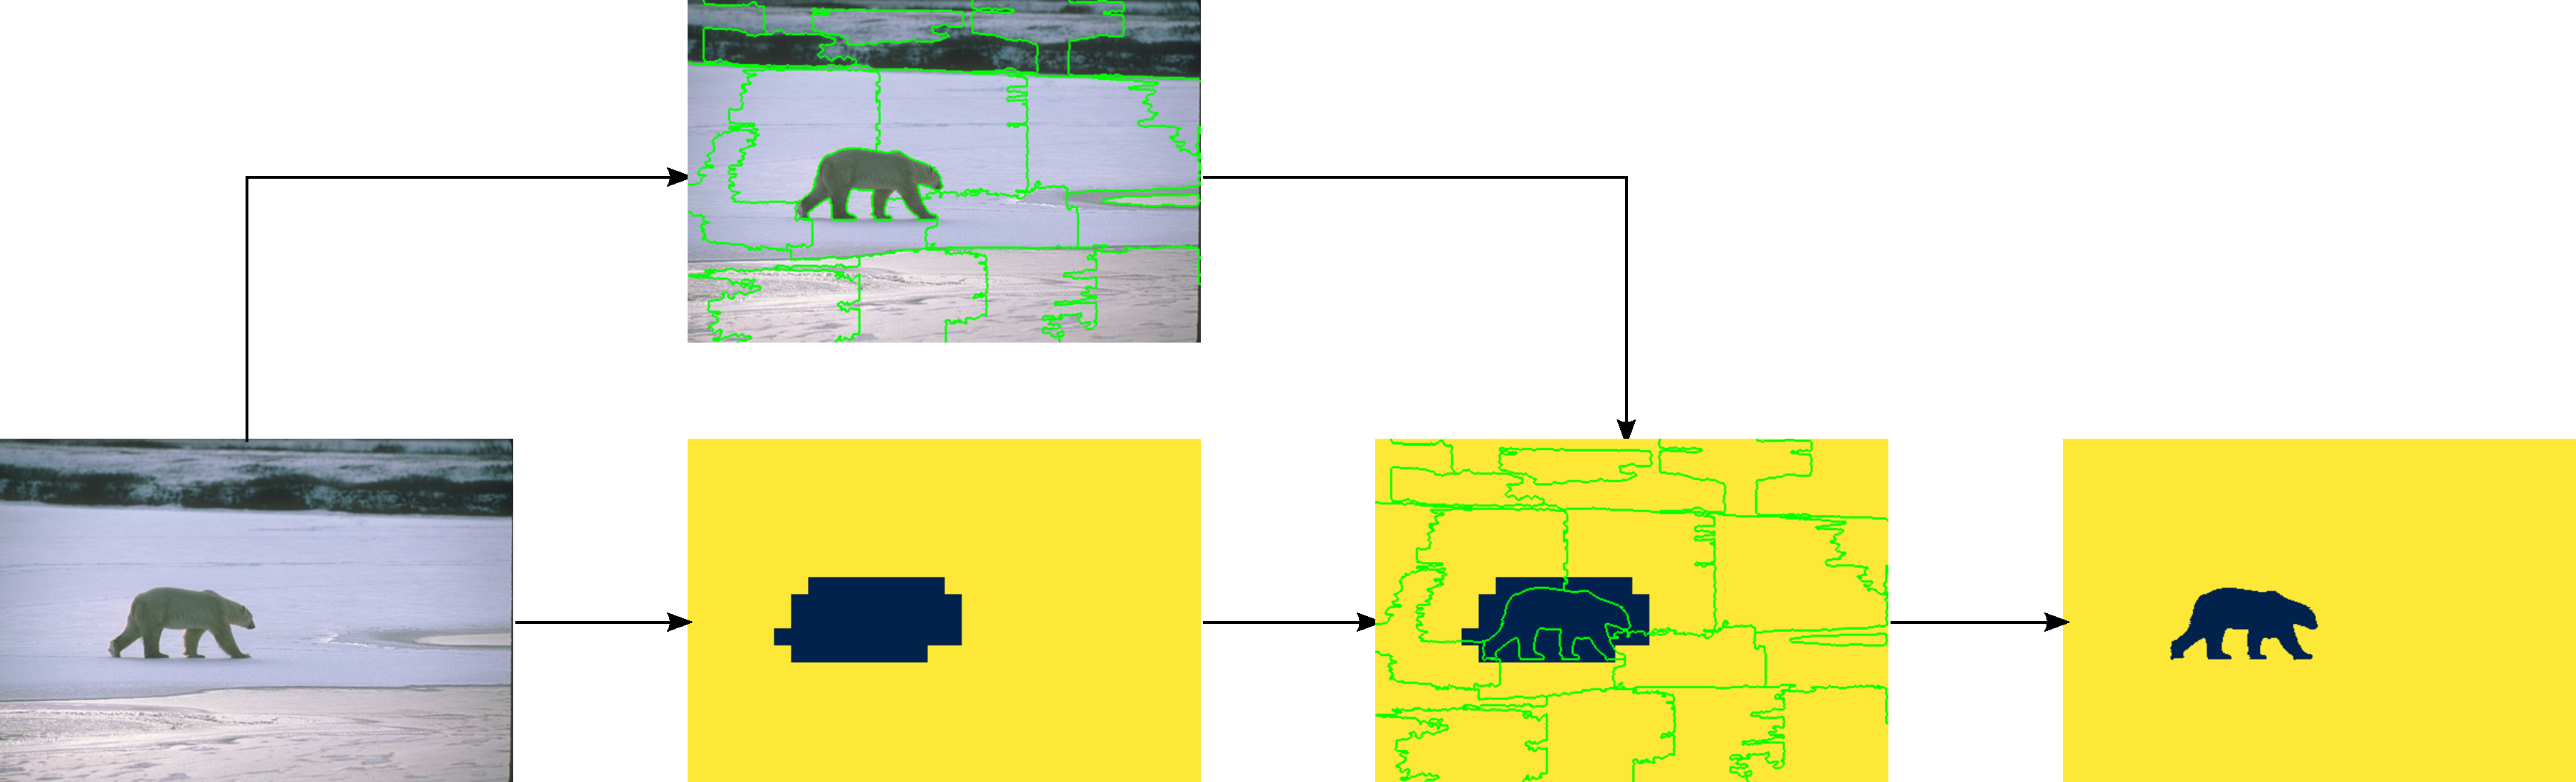
\includegraphics[width=\linewidth]{figures/smv.pdf}
    \caption{An outline of the boundary refinement process. The superpixel image is superimposed on the upsampled segmentation image. Then, each superpixel is labelled with its majority label.}
    \label{fig:smv}
\end{figure}

In order to use the superpixel image to refine the segmentation image, both images need to have the same spatial resolution. Since more accurate contours are present in the higher resolution superpixel image, the segmentation image needs to be upsampled. The segmentation image is essentially an image of cluster labels. Hence, the upsampled version of the segmented image cannot contain in-between values. Nearest Neighbour Upsampling can be used to generate the higher resolution image without introducing new pixel values in the image. Each pixel in the higher resolution image gets its value from its nearest neighbour pixel in the lower resolution image.

\emph{Superpixel Majority Voting} (SMV) is a method that uses boundary information from a superpixel color image to correct the boundaries in the label image \parencite{feng2021superpixel}. First, SMV superimposes the superpixel image on the upsampled label image. Then, it ensures that all pixels within one superpixel have the same label. It does so by labelling all the pixels within one superpixel by the majority pixel label within that superpixel (see last step in \autoref{fig:smv}). Consequently, the jagged edges present in the upsampled label disappear and the image adheres well to the boundaries present in the superpixel image.

It is important to note that the size of the superpixels plays an important role in the correction step. Larger superpixels might cover more than one region and yield an image with over-corrected boundaries. This results in parts of the foreground merging with the background. In contrast, smaller superpixels cannot significantly change the contours. This limits the amount of correction made by SMV. Thus, the final contours might be under-corrected.

Another factor that affects the SMV output is the quality of the segmentation image. SMV cannot correct a poor segmentation image where the proposed regions are too large compared to the actual size occupied by their corresponding objects in the original image. This is due to the error in the poor segmentation image being enlarged during the upsampling process before applying SMV.

%%%%%%%%%%%%%%%%%%%%%%%%%%%%%%%%%%%%%%%%%%%%%%%%%%%%%%%%%%%%%%%%%%%%
%%%%%%%%%%%%%%%%%%%%%%%%%%%%%%%%%%%%%%%%%%%%%%%%%%%%%%%%%%%%%%%%%%%%
%%%%%%%%%%%%%%%%%%%%%%%NORM%%%%%%%%%%%%%%%%%%%%%%%%%%%%%%%%%%%%%%%%%%
%%%%%%%%%%%%%%%%%%%%%%%%%%%%%%%%%%%%%%%%%%%%%%%%%%%%%%%%%%%%%%%%%%%%
%%%%%%%%%%%%%%%%%%%%%%%%%%%%%%%%%%%%%%%%%%%%%%%%%%%%%%%%%%%%%%%%%%%%
%%%%%%%%%%%%%%%%%%%%%%%%%%%%%%%%%%%%%%%%%%%%%%%%%%%%%%%%%%%%%%%%%%%%
\section{Feature Pixel Normalization}

During our segmentation experiments, we noticed that normalizing the pixels in the feature image to unit length had a significant effect on the clustering output. More specifically, the pixel lengths of the feature images extracted at the deepest convolutional layer of VGG16 often determined the clustering result. \autoref{fig:norm_test} shows the effect of normalizing feature pixels to unit length on four different images. The figure shows that the non-normalized feature pixels are clustered based on their magnitude. Feature pixels with a greater magnitude are clustered into one group while those with a lower magnitude are clustered into a second group. By normalizing the feature pixels to unit length, the pixels are clustered based on their relative instead of their combined activations in the feature maps.

\begin{figure}[!ht]
    \centering
    \includegraphics[width=\textwidth]{figures/norm_test2.pdf}
    \caption{A figure showing the effect of normalizing feature pixels to unit lengths before clustering them.}
    \label{fig:norm_test}
\end{figure}